\documentclass[a4paper, 11pt]{report}
\setcounter{tocdepth}{3}
\usepackage[utf8]{inputenc}
\usepackage[french]{babel}
\usepackage[T1]{fontenc}
\usepackage{graphicx}
\usepackage{xcolor}
\usepackage{booktabs}
\usepackage{tabularx}
\usepackage{fourier} 
\usepackage{array}
\usepackage{makecell}
\usepackage[top=2.5cm,bottom=2.5cm,right=2.5cm,left=2.5cm]{geometry}
\usepackage{amsmath}
\usepackage{xcolor}
\usepackage{colortbl,hhline}
\usepackage{subfig}
\usepackage{multirow}
\usepackage{comment}
\usepackage{makecell}

\usepackage{algorithmic,algorithm}

\renewcommand{\listalgorithmname}{Liste des \ALG@name s}

\definecolor{yacine}{RGB}{241,241,241}
\usepackage{tikz}
\def\checkmark{\tikz\fill[scale=0.4](0,.35) -- (.25,0) -- (1,.7) -- (.25,.15) -- cycle;} 

\usepackage[backend=bibtex,style=numeric,sorting=nty]{biblatex}
\nocite{*} %Ausgabe aller Bibliographieeinträges
\usepackage{hyperref}
\hypersetup{
    linktoc=all,     %set to all if you want both sections and subsections linked
}




\begin{document}
\section{Gestion d'attribut manquant} 
Exemple de gestion d'attributs à valeurs manquantes avec l'algorithme C4.5\\
Soit l'arbre de décision, ainsi que l'ensemble d'apprentissage suivants :









\begin{table}[!h]
\begin{small}
\begin{tabular}{cc}

    \begin{minipage}{.5\linewidth}
   
\begin{footnotesize}
\begin{tabular}{| l | l | l | l | l |}
\hline
Temps & Température & Humidité & Vent & Jouer \\
\hline
Ensoleillé & Haute & Haute & Faux & \cellcolor{green}Non \\
\hline
Ensoleillé & Haute & Haute & Vrai & \cellcolor{green}Non \\
\hline
Couvert & Haute & Haute & Faux & \cellcolor{yellow}Oui \\
\hline
Pluvieux & Basse & Haute & Faux & \cellcolor{yellow}Oui \\
\hline
Pluvieux & Moyenne & Normal & Faux & \cellcolor{yellow}Oui \\
\hline
Pluvieux & Moyenne & Normal & Vrai &  \cellcolor{green}Non \\
\hline
Couvert & Moyenne & Normal & Vrai &  \cellcolor{yellow}Oui \\
\hline
Ensoleillé & Basse & Haute & Faux &  \cellcolor{green}Non \\
\hline
Ensoleillé & Moyenne & Normal & Faux &  \cellcolor{yellow}Oui \\
\hline
Pluvieux & Basse & Normal & Faux &  \cellcolor{yellow}Oui \\
\hline
Ensoleillé & Basse & Normal & Vrai &  \cellcolor{yellow}Oui \\
\hline
Couvert & Basse & Haute & Vrai &  \cellcolor{yellow}Oui \\
\hline
Couvert & Haute & Normal & Faux &  \cellcolor{yellow}Oui \\
\hline
Pluvieux & Moyenne & Haute & Vrai &  \cellcolor{green}Non \\
\hline
\end{tabular}
\caption{Données d'apprentissage A}
\end{footnotesize}


      \caption{Sous ensemble F}

    \end{minipage} &

    \begin{minipage}{.5\linewidth}
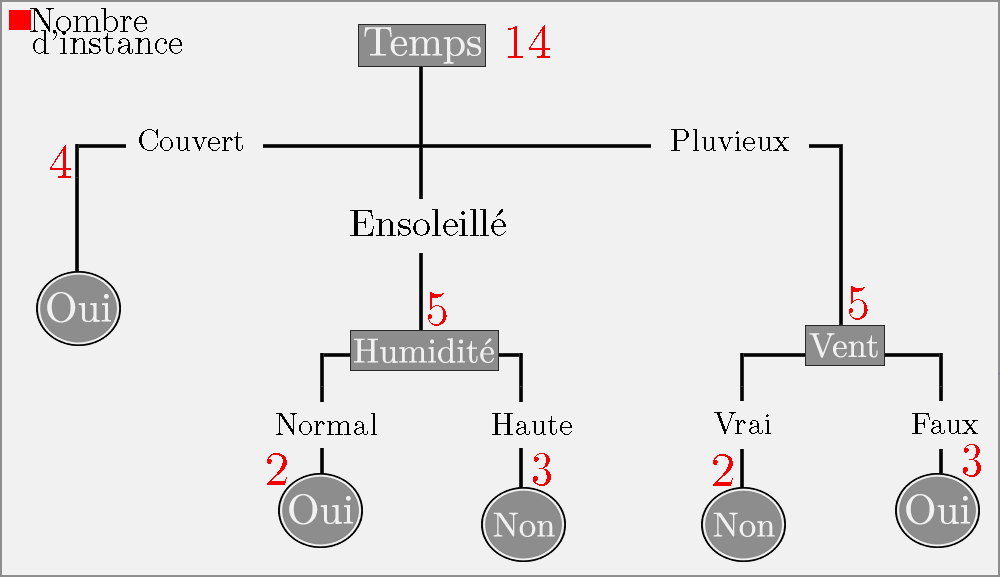
\includegraphics[scale=1.8]{figure_GI2}
\caption{L'arbre de décision correspondant aux données A}
    \end{minipage} 
\end{tabular}
\end{small}
\end{table}











Supposons que nous avons l'instance suivante a classer :\\
\begin{center}
\begin{tabular}{| c | c | c | c | c |}
\hline 
Temps & Température & Humidité & Vent & Jouer ? \\
\hline
Pluvieux & Haute & Normal & . & ? \\
\hline 
\end{tabular}
\end{center}


Supposons qu'une instance des données de teste qui a comme valeur temps "Ensoleillé", mais qui n'a pas de valeur pour l'attribut humidité.\\
En parcourant les testes de notre arbre de décision, cette instance prendra le chemin "Pluvieux", ensuite, il y aura un teste pour lequel elle a une valeur manquante.
Nous remarquons que le teste divise les données en deux sous ensemble, 2 instances corresponde au testes "vent=vrai", contre 3 instances qui correspondent au teste "vent=faux"
L'algorithme \emph{C4.5} renverrait une distribution de probabilité de [$\frac{2}{5}$,$\frac{3}{5}$]correspondante à [Non,Oui] pour cette instance à valeur manquante.

\end{document}
